%laden der Präambel mit Latexbefehlen/-klassen

\pdfmajorversion=1
\pdfminorversion=3

\documentclass[a4paper, 12pt, openany]{article}

% Font type
\usepackage[T1]{fontenc}
\usepackage{mathpazo}
\usepackage{libertine}

% laden aller packages
\usepackage{preamble}
\usepackage{setspace}
\usepackage{parskip}
\usepackage{xurl} % Sorgt für perfekte Zeilenumbrüche bei Pfaden und URLs
\usepackage{float}
\setstretch{1.1}





%%%%%%%%%%%%%%%%%%%%%%%%%%%%%%%%%%%%%%%%%%%%%%%%%%
%%%%% ~~~~~ Frontmatter - Vorderteil ~~~~~
%%%%%%%%%%%%%%%%%%%%%%%%%%%%%%%%%%%%%%%%%%%%%%%%%%

\begin{document}

% Titelseitenlayout laden
\pagestyle{empty}
% Neue Seitenränder, die nur für die Titelseite gelten
\newgeometry{top=25mm, bottom=25mm, left=25mm, right=25mm}

% Deckblatt einfügen
% !suchen Sie sich eine der Titelseiten aus!
\begin{titlepage}
    \begin{center}
        \vspace*{1.2cm}

        
\includegraphics[width=5cm]{assets/img/hs-fulda_logo_rund_gruen-schwarz_keinhintergrund_keineschutzzone_300ppi.png}\\[1.25cm]

      {\LARGE \textbf{Praxisorientierte Fallstudie:}}\\[0.6cm]

        {\Large \textbf{Nutzwertanalyse von \gls{e2etest}-Frameworks (Selenium vs. Cypress) für die Automatisierung repräsentativer regressionskritischer Testszenarien zur Reduzierung des manuellen Testaufwands}}\\[1.5cm]

        \textbf{Name:} Marcel Licht\\
        \textbf{Studiengang:} Bachelor Angewandte Informatik dual\\
        \textbf{Modul:} Aktuelles Thema der Angewandten Informatik -- Praxisorientierte Fallstudie\\
        \textbf{Matrikelnummer:} 1540372\\
        \textbf{Lehrperson:} Prof.\ Dr.\ Martine Herpers\\
        \textbf{Unternehmen:} JUMO GmbH \& Co.\ KG\\
        \textbf{Fachbetreuung:} Daniel Kircher\\
        \textbf{Datum:} \today

        \vfill

        {\large Hochschule Fulda}
    \end{center}
\end{titlepage}

% Zurück zu den Standard-Seitenrändern für KApitel und Text
% top=25mm, bottom=25mm, inner=30mm, outer=30mm, headsep=10mm, footskip=12mm
\restoregeometry

%\glsaddall

% Abstrakt
%%%%%%%%%%%%%%%%%%%%%%%%%%%%%%%%%%%%%%%%%%%%%%%%%%
%%%%		~~~~ Abstrakt ~~~~
%%%%%%%%%%%%%%%%%%%%%%%%%%%%%%%%%%%%%%%%%%%%%%%%%%
% Sollte wirklich kurz sein, 300 Wörter, maximal 500
\begin{abstract}
\justifying % Setzt den Text im Blocksatz
\noindent



Das Testen von Software, insbesondere von regressionskritischen Nutzungsszenarien, ist im Entwicklungsalltag häufig mit einem hohen manuellen und zeitintensiven Aufwand verbunden. Diese Fallstudie untersucht im Kontext der internen Webanwendung \glqq Puma\grqq\ der JUMO GmbH \& Co.\ KG, wie dieser Aufwand durch den Einsatz automatisierter End-to-End-Test-Frameworks zielgerichtet reduziert werden kann. Ziel der Arbeit ist es, auf Basis einer strukturierten Evaluierung das am besten geeignete Werkzeug für die spezifischen, stark reglementierten Unternehmensanforderungen zu identifizieren. Hierfür werden die etablierten Frameworks Selenium und Cypress einander gegenübergestellt.

Die methodische Untersuchung kombiniert eine prototypische Implementierung dreier repräsentativer Testszenarien mit einer anschließenden Nutzwertanalyse nach Kühnapfel. Die Bewertung erfolgt anhand von fünf betrieblich gewichteten Kriterien: Integration in die Infrastruktur (25\,\%), Lernkurve und Syntax (20\,\%), Test-Ausführung und Debugging (20\,\%), Stabilität (20\,\%) sowie Dokumentation und Ökosystem (15\,\%).

Die Ergebnisse der Analyse zeigen, dass Cypress mit einem Gesamtnutzwert von 7,800 aus rein entwicklungstechnischer Sicht dem Framework Selenium (7,200) überlegen ist. Cypress punktet maßgeblich durch eine intuitivere Syntax und signifikant höhere Teststabilität dank integriertem Auto-Waiting. Dennoch offenbart die prototypische Umsetzung gravierende infrastrukturelle Hürden für Cypress: Strenge Proxy-Vorgaben und das etablierte Java-Ökosystem des Unternehmens erschweren eine nahtlose Einbindung erheblich. Selenium lässt sich hingegen als Java-Bibliothek sofort und reibungslos in den bestehenden Maven-Buildprozess integrieren.

Aus diesen Erkenntnissen wird die Handlungsempfehlung abgeleitet, kurzfristig Selenium für die Automatisierung der Tests zu nutzen, um zeitnah erste Automatisierungsgewinne zu erzielen. Mittelfristig sollte das Unternehmen jedoch prüfen, ob die CI/CD-Infrastruktur für Node.js-Umgebungen geöffnet werden kann, um zukünftig von der technischen Überlegenheit von Cypress zu profitieren.

\end{abstract}
\clearpage

% Inhaltsverzeichnis
\begin{spacing}{1.3}
\tableofcontents
\clearpage

% Abbildungsverzeichnis
\phantomsection % Fügt einen unsichtbaren Abschnitt hinzu, um den Link zu korrigieren
\addcontentsline{toc}{section}{\listfigurename}
\listoffigures
\clearpage

% Tabellenverzeichnis
\phantomsection % Fügt einen unsichtbaren Abschnitt hinzu, um den Link zu korrigieren
\addcontentsline{toc}{section}{\listtablename}
\listoftables
\clearpage

% Listingverzeichnis
\phantomsection % Fügt einen unsichtbaren Abschnitt hinzu, um den Link zu korrigieren
\addcontentsline{toc}{section}{Quellcodeverzeichnis}
\lstlistoflistings
\clearpage

\end{spacing}

%%%%%%%%%%%%%%%%%%%%%%%%%%%%%%%%%%%%%%%%%%%%%%%%%%
%%%%% ~~~~~ Mainmatter - Hauptteil Text ~~~~~
%%%%%%%%%%%%%%%%%%%%%%%%%%%%%%%%%%%%%%%%%%%%%%%%%%
\pagestyle{plain}
\justifying
\setlength{\parindent}{0pt}

% Einfügen aller Kapitel
% --------------------------------------------------
% 1. Einleitung
% --------------------------------------------------
\section{Einleitung}

\subsection{Problemstellung und Motivation}
Das Testen von Software ist ein zentraler Bestandteil moderner Softwareentwicklung, um funktionale Anforderungen und einen zuverlässigen Betrieb von Anwendungen sicherzustellen. Historisch wurden Tests überwiegend manuell durchgeführt. Mit der zunehmenden Komplexität heutiger Softwaresysteme und steigenden Anforderungen an Entwicklungsgeschwindigkeit hat sich jedoch der Einsatz automatisierter Testverfahren etabliert \cite{spillner2024basiswissen}.

Im betrieblichen Kontext der JUMO GmbH \& Co.\ KG wird die intern entwickelte Java-Webanwendung \glqq Puma\grqq\ (auch \glqq Workspace\grqq\ genannt) zur Prozessverwaltung fortlaufend durch Fehlerbehebungen und neue Funktionen erweitert. Trotz der Relevanz automatisierter Tests erfolgen die Prüfungen zentraler Nutzungsszenarien derzeit noch überwiegend manuell -- zunächst durch die Entwickler im Testsystem und anschließend als Abnahmetest durch die anfordernden Fachabteilungen. Dies geschieht häufig in Form explorativer Tests.

Dieser manuelle Testaufwand ist zeitintensiv, bindet personelle Ressourcen auf beiden Seiten und erschwert eine strukturierte Absicherung von Änderungen. Zudem schwanken die Testergebnisse stark je nach durchführender Person, was die Reproduzierbarkeit einschränkt. Vor diesem Hintergrund entsteht der Bedarf, geeignete Ansätze zur teilweisen Automatisierung regressionskritischer End-to-End-Tests (E2E-Tests) systematisch zu untersuchen -- also jener Testszenarien, die nach Änderungen besonders anfällig für unerwünschte Seiteneffekte sind. 

Erschwerend müssen bei der Werkzeugauswahl spezifische infrastrukturelle Rahmenbedingungen der JUMO GmbH \& Co.\ KG berücksichtigt werden. Dazu zählen die bestehende Entwicklungslandschaft (älteres JDK, Eclipse, Maven) sowie strikte Proxy- und Netzwerksperren des Unternehmens. Im Fokus dieser Arbeit stehen daher die E2E-Frameworks Selenium \cite{Selenium} und Cypress \cite{Cypress}.

Die Motivation der Arbeit ergibt sich somit aus dem konkreten betrieblichen Bedarf, die Qualitätssicherung bei häufigen Softwareänderungen effizienter und reproduzierbarer zu gestalten. 

\subsection{Zielsetzung der Arbeit}
Ziel der vorliegenden Fallstudie ist es, auf Basis eines strukturierten Vergleichs eine fundierte Entscheidungshilfe für die Auswahl eines End-to-End-Test-Frameworks bei der JUMO GmbH \& Co.\ KG zu erarbeiten. 

Dabei ist es nicht das Ziel, ein allgemein überlegenes Framework zu bestimmen, sondern das Werkzeug zu identifizieren, welches für den konkreten Unternehmenskontext und dessen technische Restriktionen am besten geeignet ist. Hierzu werden relevante Anforderungen aus dem Betrieb abgeleitet, ausgewählte Nutzungsszenarien der \glqq Puma\grqq-Webanwendung prototypisch in beiden Frameworks umgesetzt und die Ergebnisse anhand einer Nutzwertanalyse systematisch bewertet.

\subsection{Forschungsfrage und Aufbau der Arbeit}
Aus der formulierten Zielsetzung leitet sich die zentrale Forschungsfrage dieser Fallstudie ab:

\begin{quote}
\textit{Welches der beiden Frameworks (Selenium oder Cypress) ist für die Automatisierung ausgewählter repräsentativer regressionskritischer End-to-End-Testszenarien im gegebenen Unternehmenskontext besser geeignet, wenn Integrationsaufwand, Wartbarkeit, Stabilität, Ausführungseffizienz und Unterstützungsangebote systematisch berücksichtigt werden?}
\end{quote}

Zur präzisen Beantwortung der Hauptfrage werden folgende Teilfragen untersucht:
\begin{itemize}
    \item Welche Anforderungen ergeben sich aus dem betrieblichen Umfeld an ein End-to-End-Test-Framework?
    \item Welche Nutzungsszenarien der Webanwendung eignen sich als repräsentative Testfälle für einen Framework-Vergleich?
    \item Wie unterscheiden sich Selenium und Cypress hinsichtlich des technischen und organisatorischen Integrationsaufwands?
    \item Welche Unterschiede zeigen sich in Bezug auf Verständlichkeit, Wartbarkeit und Änderbarkeit des Testcodes?
    \item Wie unterscheiden sich die Frameworks bezüglich Stabilität, Laufzeit und Diagnosemöglichkeiten im Fehlerfall?
\end{itemize}

\textbf{Aufbau der Arbeit:}\\
Im Anschluss an diese Einleitung werden in Kapitel 2 die theoretischen Grundlagen des End-to-End-Testings sowie der untersuchten Frameworks Selenium und Cypress erläutert. 
Kapitel 3 widmet sich der Methodik und beschreibt das Vorgehen der Nutzwertanalyse inklusive der Entwicklung des Kriterienmodells. 
In Kapitel 4 erfolgt die Beschreibung der prototypischen Umsetzung und der Datenerhebung anhand der ausgewählten Testszenarien. 
Kapitel 5 präsentiert die Auswertung der Ergebnisse mittels der Nutzwertanalyse. Die Arbeit schließt in Kapitel 6 mit einer Diskussion der Erkenntnisse und einem zusammenfassenden Fazit.

\clearpage
% --------------------------------------------------
% 2. Theoretische Grundlagen
% --------------------------------------------------
\section{Theoretische Grundlagen}

Dieses Kapitel legt das theoretische Fundament für die Fallstudie. Es beleuchtet zunächst den aktuellen Stand der Forschung, definiert die Rolle von \gls{e2etests} in der Qualitätssicherung, stellt anschließend die beiden zu vergleichenden Frameworks vor und erläutert abschließend die Methodik der Nutzwertanalyse.

\subsection{Stand der Forschung}
Die Evaluierung und der Vergleich von Testautomatisierungswerkzeugen sind Gegenstand zahlreicher Publikationen der angewandten Informatik. Während grundlegende Werke wie Liggesmeyer \cite{Liggesmeyer2009} oder Spillner und Linz \cite{spillner2024basiswissen} die theoretischen Konzepte des Softwaretests und der Testautomatisierung umfassend behandeln, fokussieren sich neuere Publikationen häufig auf den Architekturvergleich spezifischer Frameworks. Der Kontrast zwischen traditionellen \gls{webdriver}-basierten Ansätzen wie Selenium und modernen, browserinternen Werkzeugen wie Cypress wird in der Fachliteratur oft anhand von Metriken wie Ausführungsgeschwindigkeit, Stabilität (Flakiness) und \gls{api}-Design diskutiert. 

Eine Lücke besteht jedoch oft in der detaillierten Betrachtung dieser Tools innerhalb stark reglementierter Unternehmensnetzwerke und spezifischer Legacy-Infrastrukturen (wie z.\,B. ältere \gls{jdk}-Versionen oder strikte Proxy-Vorgaben). Die vorliegende Fallstudie knüpft an den bestehenden Forschungsstand an, erweitert ihn jedoch um eine systematische Bewertung, die exakt diese praxisnahen infrastrukturellen und organisatorischen Rahmenbedingungen der JUMO GmbH \& Co. KG in den Mittelpunkt stellt.

\subsection{Softwaretest und \gls{e2etest}ing}
Die Testautomatisierung ist ein fest etablierter Bestandteil moderner Softwarequalitätssicherung \cite{Liggesmeyer2009}. Während Unit- und Integrationstests isolierte Code-Abschnitte oder Schnittstellen auf technischer Ebene prüfen, testen \gls{e2etests} (\gls{e2e}-Tests) das gesamte System über alle Schichten hinweg -- von der Benutzeroberfläche bis zur Datenbank. Sie dienen insbesondere dazu, regressionskritische Nutzungsszenarien aus Sicht der Endanwender in einer realitätsnahen Umgebung zu überprüfen und dadurch zentrale Geschäftsprozesse abzusichern \cite{spillner2024basiswissen}. Da \gls{e2e}-Tests in der Regel komplexer in der Einrichtung und laufzeitintensiver sind, ist die Wahl eines robusten, wartbaren und in die Systemlandschaft passenden Automatisierungs-Frameworks entscheidend für die langfristige Akzeptanz im Entwicklungsalltag.

\subsection{Betrachtete Test-Frameworks: Selenium und Cypress}
Für den praktischen Vergleich dieser Arbeit stehen die Werkzeuge Selenium und Cypress im Mittelpunkt.

\textbf{Selenium} ist ein langjährig etabliertes Standardwerkzeug der browserbasierten Testautomatisierung. Es steuert den Browser über das native \gls{webdriver}-Protokoll an und bietet breite Integrationsmöglichkeiten in unterschiedliche Programmiersprachen, wie beispielsweise Java \cite{Selenium}. Diese hohe Flexibilität und Rückwärtskompatibilität erfordern jedoch im Gegenzug oftmals einen höheren manuellen Konfigurationsaufwand, insbesondere bei der Handhabung von asynchronen Ladezeiten und der Synchronisation des Testablaufs.

\textbf{Cypress} wird demgegenüber häufig als moderne, entwicklerzentrierte Alternative für Webanwendungen herangezogen. Im Gegensatz zu Selenium läuft Cypress direkt im Browser und führt Tests in derselben Event-Loop wie die Anwendung selbst aus \cite{Cypress}. Dies ermöglicht eine direkte Rückmeldung während der Testausführung, ein automatisches Warten auf \gls{dom}-Elemente (\textit{\gls{autowaiting}}) sowie sehr gute Debugging-Möglichkeiten. Da Cypress jedoch primär auf JavaScript beziehungsweise TypeScript ausgelegt ist, bedarf es bei der Integration in bestehende Java-Ökosysteme oder stark reglementierte Firmennetzwerke einer gesonderten Betrachtung.

Der Mehrwert der vorliegenden Arbeit liegt demnach nicht in einer rein allgemeinen Toolbeschreibung, sondern in der kontextbezogenen Bewertung dieser Frameworks für konkrete Webanwendungen unter realen infrastrukturellen Restriktionen im Unternehmensumfeld.

\subsection{Nutzwertanalyse als Bewertungsmethode}
Zur strukturierten und objektiven Entscheidungsfindung wird die Nutzwertanalyse verwendet. Diese Methode erlaubt es, mehrere Handlungsalternativen anhand systematisch gewichteter qualitativer und quantitativer Kriterien nachvollziehbar zu vergleichen \cite{Kuehnapfel2021}. Das Verfahren gliedert sich in vier zentrale Schritte: die Definition der relevanten Bewertungskriterien, deren Gewichtung auf Basis der betrieblichen Anforderungen, die Ermittlung der Zielerfüllung (Punktevergabe) durch prototypische Messungen sowie die finale Berechnung des Gesamtnutzwertes. Damit wird ein bestehender praktischer Bedarf mit einer methodisch fundierten Bewertungslogik verbunden, um eine kontextbezogene Entscheidungshilfe abzuleiten.
% --------------------------------------------------
% 3. Methodisches Vorgehen
% --------------------------------------------------
\section{Methodisches Vorgehen}
\label{sec:methodik}

Um die Eignung der Frameworks Selenium und Cypress für den Einsatz bei der JUMO GmbH \& Co.\ KG systematisch und objektiv zu vergleichen, wurde ein praxisorientiertes Forschungsdesign gewählt. Dieses Kapitel beschreibt den methodischen Aufbau der Fallstudie, die Auswahl der Testszenarien, die Definition der Bewertungskriterien sowie den Ablauf der praktischen Erprobung.

\subsection{Forschungsdesign der Fallstudie}
Die Untersuchung basiert auf einer Kombination aus prototypischer Implementierung und einer strukturierten Entscheidungsfindung mittels Nutzwertanalyse (NWA) nach Kühnapfel \cite{Kuehnapfel2021}. 
Da ein rein theoretischer Vergleich der Frameworks den spezifischen infrastrukturellen Kontext des Unternehmens nicht ausreichend berücksichtigen würde, werden beide Werkzeuge in der realen Entwicklungsumgebung erprobt. 

Die Ergebnisse dieser praktischen Umsetzung fließen in die Nutzwertanalyse ein. Diese Methode erlaubt es, qualitative und quantitative Beobachtungen in messbare Punktwerte zu übersetzen, diese mit unternehmensspezifischen Gewichtungen zu versehen und so zu einem nachvollziehbaren Gesamtergebnis zu gelangen.

\subsection{Auswahl repräsentativer regressionskritischer Testszenarien}
Da eine vollständige Automatisierung aller Anwendungsfälle der \glqq Puma\grqq-Webanwendung den Rahmen dieser Studie sprengen würde, wurden repräsentative und regressionskritische Nutzungsszenarien ausgewählt. Diese Szenarien bilden die Kernfunktionalitäten der Anwendung ab und sind nach funktionalen Erweiterungen besonders fehleranfällig. 

Für die prototypische Umsetzung wurden folgende drei Szenarien definiert:

\subsection{Auswahl repräsentativer regressionskritischer Testszenarien}
Da eine vollständige Automatisierung aller Anwendungsfälle der \glqq Puma\grqq-Webanwendung den Rahmen dieser Studie sprengen würde, wurden repräsentative und regressionskritische Nutzungsszenarien ausgewählt. Diese Szenarien bilden die Kernfunktionalitäten der Anwendung ab und sind nach funktionalen Erweiterungen besonders fehleranfällig. 

Für die prototypische Umsetzung wurden folgende drei Szenarien definiert:
\begin{enumerate}
    \item \textbf{Authentifizierung:} Ein Login-Vorgang zur Prüfung des Zugriffs auf geschützte Bereiche. Obwohl dieser Bereich bei funktionalen Erweiterungen der Anwendung selten direkt modifiziert wird, ist er aufgrund seiner hohen Kritikalität (Totalausfall bei Defekt) zwingend abzusichern. Zudem dient er im Framework-Vergleich als methodische Baseline zur Evaluation grundlegender Interaktions- und Warte-Mechanismen ohne überlagernde Geschäftslogik.
    
    \item \textbf{Formularverarbeitung:} Das Ausfüllen, Validieren und Absenden eines typischen Eingabeformulars. Formulare stellen einen zentralen Interaktionspunkt der Anwendung dar. Dieses Szenario eignet sich besonders, um zu vergleichen, wie die Frameworks mit verschiedenen UI-Elementen (wie Dropdowns oder Pflichtfeldern) sowie mit der Auswertung von Validierungsmeldungen im Browser umgehen.
    
    \item \textbf{Datensatzbearbeitung:} Ein mehrstufiger Prozess, bei dem ein Datensatz aufgerufen, modifiziert, gespeichert und die erfolgreiche Änderung im Anschluss verifiziert wird. Da die Prozessverwaltung den fachlichen Kernbereich der Anwendung darstellt, sind solche Abläufe nach Updates stark regressionsgefährdet. Dieses komplexe Szenario testet primär, wie zuverlässig die Werkzeuge asynchrone Ladezeiten (z.\,B. Warten auf das Speichern im Backend) und die zusammenhängende Navigation über mehrere Ansichten hinweg handhaben.
\end{enumerate}

\subsection{Ableitung und Gewichtung der Bewertungskriterien}
Die Bewertungskriterien für die Nutzwertanalyse wurden direkt aus den fachlichen, technischen und organisatorischen Anforderungen des Ausbildungsbetriebs abgeleitet. Um der betrieblichen Realität gerecht zu werden, wurden folgende Hauptkriterien definiert:

\begin{itemize}
    \item \textbf{Integrationsaufwand:} Bewertung der initialen Einrichtung innerhalb der bestehenden Infrastruktur. Hierbei spielen insbesondere das vorhandene Build-Management (Maven), das genutzte JDK sowie der Umgang mit den strikten Proxy- und Netzwerksperren des Unternehmens eine zentrale Rolle.
    \item \textbf{Verständlichkeit und Wartbarkeit:} Beurteilung der Syntax und Struktur des Testcodes. Es wird bewertet, wie schnell sich neue Entwickler einarbeiten können und wie aufwendig die Pflege der Tests bei zukünftigen UI-Anpassungen ist.
    \item \textbf{Stabilität und Laufzeit:} Analyse der Ausführungsgeschwindigkeit sowie der Zuverlässigkeit der Tests (z.\,B. Anfälligkeit für sogenannte \textit{Flaky Tests}, die sporadisch ohne Code-Änderung fehlschlagen).
    \item \textbf{Fehlerdiagnose und Dokumentation:} Bewertung der Möglichkeiten zur Fehlersuche (Debugging, Screenshots/Videos bei Fehlschlägen) sowie der Qualität der offiziellen Dokumentation und Community-Unterstützung.
\end{itemize}
Die Gewichtung dieser Kriterien erfolgt vor dem Hintergrund der Unternehmensziele: Da die Tests von den Entwicklern lokal ausgeführt werden sollen, erhalten Integrationsaufwand und Wartbarkeit eine entsprechend hohe Priorität.

\subsection{Vorgehen der prototypischen Umsetzung}
Die praktische Erprobung erfolgt schrittweise. Zunächst wird für beide Frameworks eine lokale Testumgebung aufgesetzt. Dabei wird dokumentiert, welche Konfigurationsschritte und Workarounds (beispielsweise bei Abhängigkeiten-Downloads über den Firmen-Proxy) notwendig sind.

Anschließend werden die drei definierten Testszenarien (Login, Formular, Datensatzbearbeitung) nacheinander zunächst in Selenium und danach in Cypress implementiert. Um eine Vergleichbarkeit zu gewährleisten, wird für beide Frameworks derselbe Ausgangszustand der Anwendung genutzt. Während der Entwicklung wird notiert, wie viel Aufwand für das Auffinden von Web-Elementen (DOM-Selektoren), den Umgang mit asynchronen Ladezeiten und den Aufbau der Assertion-Logik (Prüfung der erwarteten Ergebnisse) benötigt wird.

\subsection{Datenerhebung und Auswertung}
Die Datenerhebung findet parallel zur prototypischen Umsetzung statt. Quantitative Daten wie die Dauer der Testausführung und die Zeilenanzahl des Testcodes (als Indikator für Komplexität) werden direkt gemessen. Qualitative Daten, wie die Qualität der Fehlermeldungen oder Hürden bei der Netzwerkintegration, werden in Form eines Entwicklertagebuchs strukturiert festgehalten.

Nach Abschluss der Implementierung werden die erhobenen Daten in das Kriterienmodell der Nutzwertanalyse überführt. Jedes Framework erhält pro Kriterium eine Bewertung auf einer Skala von 1 bis 10. Diese Punktzahl wird mit der zuvor definierten Gewichtung multipliziert. Die Summe aller gewichteten Punkte ergibt den Gesamtnutzwert, welcher als fundierte Entscheidungsgrundlage für die abschließende Handlungsempfehlung im Fazit dient.
\section{Implementierung und Durchführung der Prototypen}
\label{ch:implementierung}

Dieses Kapitel stellt die praktische Testumgebung, die ausgeführten Testszenarien sowie den technischen und syntaktischen Vergleich zwischen Selenium und Cypress dar. Die Ausformulierung stellt dabei konkrete Projektbezüge zur Webanwendung Puma bei der JUMO GmbH \& Co. KG her.

\subsection{Testumgebung und Rahmenbedingungen}
\label{sec:testumgebung}

Die Tests wurden im betrieblichen Kontext der JUMO GmbH \& Co. KG durchgeführt. Untersuchungsgegenstand ist die interne Webanwendung \textit{Puma}, die aus einem konkreten betrieblichen Bedarf heraus entstanden ist. Da die vorherige Verwaltung firmeninterner Projekte zunehmend unübersichtlich und schwer nachvollziehbar wurde, dient Puma nun als zentrale Lösung zur Projekt- und Kostenverwaltung. Ein Projekt entspricht in der Anwendung im Wesentlichen einem Arbeitsplan, der um eine detaillierte Kosten- und Stundenplanung erweitert wurde. Darüber hinaus bietet das System Funktionen gängiger Projektplanungstools: Es lassen sich Personen und Teams zuordnen, relevante Dokumente zentral hinterlegen und Projektdaten über eine Schnittstelle direkt mit dem SAP-System synchronisieren.

Das in Abbildung \textbf{\ref{fig:uml_komponenten}} dargestellte vereinfachte Komponentendiagramm veranschaulicht die fachliche und technische Struktur der Anwendung. Im Mittelpunkt steht die Projektverwaltung als zentrale Entität. Ein Projekt ist mit Modulen für Kosten- und Stundenplanungen, Ressourcen, Teams sowie der Dokumentenverwaltung verknüpft. Zur Sicherstellung der Nachvollziehbarkeit von Änderungen werden Aktivitäten, Kommentare, Benachrichtigungen und Historieneinträge erfasst. Die Suchfunktionen werden über Apache Solr abgebildet. Technische Basisdienste wie Logging, Caching, Fehlerbehandlung und allgemeine Hilfsklassen unterstützen die fachlichen Komponenten im Hintergrund.

Der Technologie-Stack der Anwendung basiert auf Java. Als Entwicklungsumgebung kam Eclipse zum Einsatz, während Maven für das Build-Management verwendet wurde. Die Bereitstellung der Anwendung für die lokale Testausführung erfolgte über einen lokalen Tomcat-Server. Der verwendete Port für die Testausführung ist \textbf{8082}. Ohne diesen laufenden Tomcat-Server ist keine Testausführung möglich, da die Webanwendung lokal ansonsten nicht erreichbar ist.

Die Ausführung der Tests unterlag den strengen Sicherheitsrichtlinien des Firmennetzwerks. Aufgrund der unternehmensinternen Proxy-Vorgaben war die Installation externer Komponenten (wie beispielsweise npm-Pakete für Node.js) nur eingeschränkt möglich. 

Die Tests wurden lokal auf einem Entwickler-Laptop durchgeführt. Die Spezifikationen des Systems lauten wie folgt:
\begin{itemize}
    \item \textbf{Betriebssystem:} Windows 11 Enterprise
    \item \textbf{Version:} 24H2
    \item \textbf{Installationsdatum:} 29.08.2025
    \item \textbf{Betriebssystembuild:} 26100.8457
\end{itemize}
% TODO: Genaue Hardwaredaten des Entwickler-Laptops ergänzen (CPU, RAM)

Für die Testdurchführung wurde ausschließlich der Browser Microsoft Edge in der Version 120 verwendet.

\begin{figure}[htbp]
    \centering
    \fbox{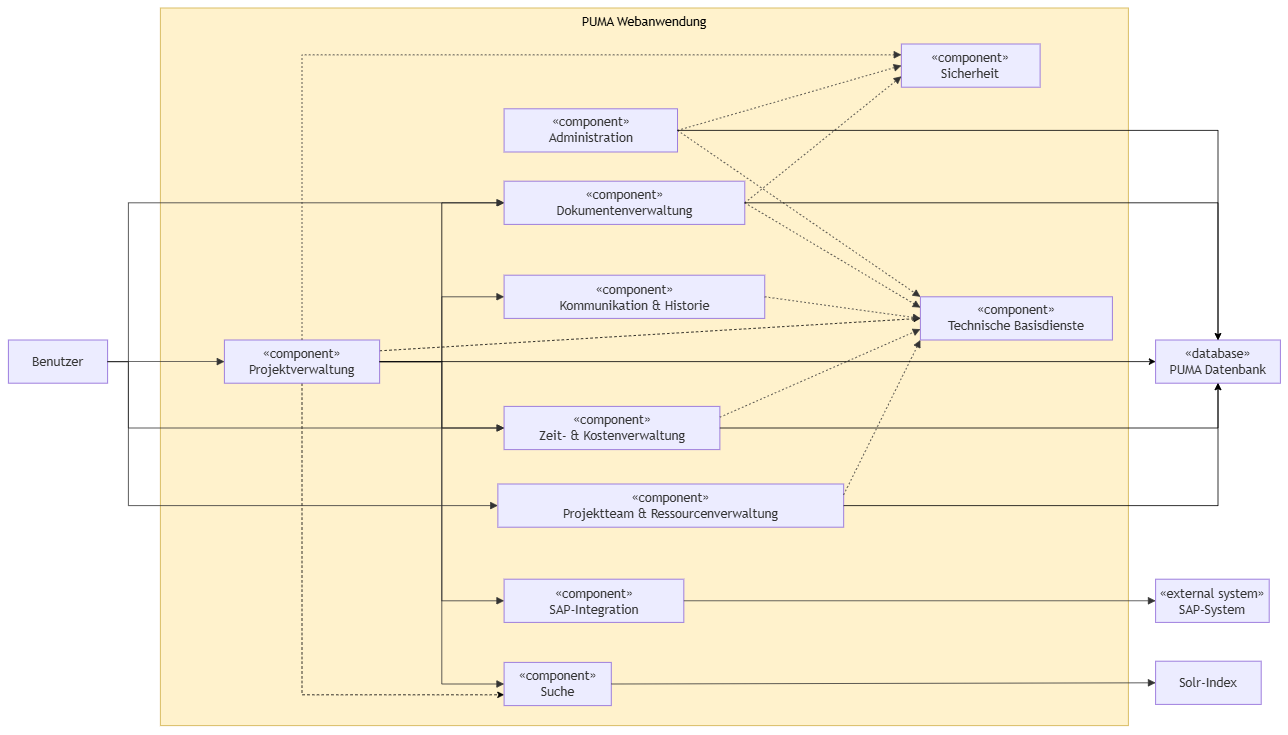
\includegraphics[width=1\textwidth]{assets/img/REALUMLFallPrax.png}}
    \caption{Fachliche und technische Struktur der Webanwendung Puma}
    \label{fig:uml_komponenten}
\end{figure}


\subsection{Beschreibung der Testszenarien}
\label{sec:testszenarien}

Dieses Unterkapitel beschreibt die getesteten Anwendungsszenarien systematisch und ordnet diese den jeweiligen Testklassen aus Selenium und den Testdateien aus Cypress zu.

\subsubsection{Szenario 1: Login}
Das Ziel dieses Tests ist es zu prüfen, ob sich ein Benutzer erfolgreich an der Puma-Webanwendung anmelden kann. Die Startbedingungen setzen voraus, dass Puma lokal über den Tomcat-Server auf Port \textbf{8082} erreichbar ist und ein gültiger Benutzer mit Benutzername und Passwort zur Verfügung steht.

Der Ablauf des Tests beginnt mit dem Öffnen der Login-Seite. Nach der Eingabe von Benutzername und Passwort wird der Login-Button betätigt. Anschließend wird geprüft, ob eine Weiterleitung auf die erwartete Zielseite erfolgt.

Das erwartete Ergebnis ist, dass der Benutzer erfolgreich angemeldet wird. Die Anwendung leitet auf die korrekte Folgeseite weiter, wobei dieser Redirect im Test validiert wird.

\textbf{Zuordnung der Testdateien:}
\begin{itemize}
    \item \textbf{Selenium:} \\ 
    \path{/ui-tests/src/test/java/ui/pumaTests/_login_Test/_01_PumaLoginTest.java}
    \item \textbf{Cypress:} \\ 
    \path{/my-springboot-app-e2e/cypress/e2e/Jumo Tests/Puma_login/01_login-ui.cy.js}
\end{itemize}


\subsubsection{Szenario 2: Neues Projekt bzw. neue Aktivität anlegen}
In diesem Szenario wird geprüft, ob ein neues Projekt bzw. eine neue Aktivität korrekt über die Benutzeroberfläche angelegt werden kann. Als Startbedingung muss der Benutzer erfolgreich angemeldet sein. Zudem muss die Anwendung lokal erreichbar sein und die benötigten Dropdown-Werte müssen im System zur Verfügung stehen.

Der Test navigiert zur Maske für die Projekt- bzw. Aktivitätsanlage. Dort wird das Stammblatt durch Eingabe der benötigten Projektdaten ausgefüllt und es werden relevante Werte in Dropdown-Feldern ausgewählt. Eine Besonderheit bilden hier Dropdowns mit \textbf{select2}, die dynamisch reagieren und daher gezielt im Code angesprochen werden müssen. Nach dem Ausfüllen wird das Formular gespeichert und die Systemrückmeldung geprüft.

Als erwartetes Ergebnis wird das Projekt oder die Aktivität erfolgreich angelegt. Die Anwendung zeigt eine korrekte Bestätigung oder Systemmeldung an, und die eingegebenen Daten sind anschließend im System vorhanden.

\textbf{Zuordnung der Testdateien:}
\begin{itemize}
    \item \textbf{Selenium:} \\ 
    \path{/ui-tests/src/test/java/ui/pumaTests/new_Activity/_02_NewActivityAnlegenTest.java} \\
    \path{/ui-tests/src/test/java/ui/pumaTests/new_Projekt/_02_NewProjektTest.java}
    \item \textbf{Cypress:} \\ 
    \path{/my-springboot-app-e2e/cypress/e2e/Jumo Tests/Puma_new_Activity(form Fill)/02_newActivity.cy.js} \\
    \path{/my-springboot-app-e2e/cypress/e2e/Jumo Tests/Puma_new_Projekt(Form_fill)/02_newProjekt.cy.js}
\end{itemize}


\subsubsection{Szenario 3: Aktivität bearbeiten}
Das Ziel des dritten Szenarios ist die Prüfung, ob eine bestehende Aktivität geöffnet, geändert, gespeichert und anschließend korrekt validiert werden kann. Die Startbedingungen erfordern, dass der Benutzer angemeldet ist, bereits eine bestehende Aktivität vorhanden ist und diese über die Benutzeroberfläche aufgerufen werden kann.

Der Ablauf sieht die Navigation zur bestehenden Aktivität sowie das Öffnen der Bearbeitungsansicht vor. Es folgt die Änderung definierter Werte, wie beispielsweise des Fortschritts oder des Datums. Nach dem Speichern der Änderungen wird die Aktivität erneut aufgerufen, um zu validieren, ob die Änderungen korrekt übernommen wurden.

Es wird erwartet, dass die Aktivität erfolgreich gespeichert wird und die geänderten Werte korrekt in der Oberfläche angezeigt werden. Die anschließende Kontrollprüfung muss die Bearbeitung bestätigen.

\textbf{Zuordnung der Testdateien:}
\begin{itemize}
    \item \textbf{Selenium:} \\ 
    \path{/ui-tests/src/test/java/ui/pumaTests/_edit_Data/_03_ControlEditedActivityTest.java} \\
    \path{/ui-tests/src/test/java/ui/pumaTests/_edit_Data/_03_EditActivityTest.java}
    
    \item \textbf{Cypress:} \\ 
    \path{/my-springboot-app-e2e/cypress/e2e/Jumo Tests/Puma_Edit_Data/03_controlEditedActivity.cy.js} \\
    \path{/my-springboot-app-e2e/cypress/e2e/Jumo Tests/Puma_Edit_Data/03_editActivity.cy.js}
\end{itemize}


\subsection{Setup und technische Integration}
\label{sec:setup}

Dieses Unterkapitel erläutert, wie Selenium und Cypress technisch in die bestehende Entwicklungsumgebung integriert wurden und welche spezifischen Herausforderungen dabei aufgetreten sind.

\subsubsection{Selenium}
Selenium wurde als Bibliothek in die bestehende Java-Umgebung integriert. Die Einbindung erfolgte unkompliziert über die \textbf{pom.xml} mit Maven. Da im Projekt ohnehin mit Java, Eclipse und Maven gearbeitet wird, passt das Framework sehr gut zur bestehenden Entwicklungsumgebung. Die Integration verlief weitgehend reibungslos. Ein anfängliches Kompatibilitätsproblem mit der im Unternehmen verwendeten älteren JDK-Version konnte umgangen werden.

Selenium ließ sich aufgrund der bestehenden Java- und Maven-Struktur gut in die vorhandene Entwicklungsumgebung integrieren.

\subsubsection{Cypress}
Im Gegensatz zur etablierten Java-basierten Integration von Selenium setzt Cypress eine Node.js- und npm-Umgebung voraus. Im vorliegenden Unternehmenskontext erwies sich diese technologische Anforderung als erste Hürde: Strikte Proxy- und Sicherheitsrichtlinien blockierten die reguläre Paketinstallation über npm, weshalb eine dedizierte IT-Freigabe zwingend erforderlich war.

Zwar kann eine lokale Installation über ein ZIP-Archiv als kurzfristiger Workaround dienen, dieser Ansatz wurde jedoch verworfen. Er eignet sich nicht für wiederholbare, skalierbare Continuous-Integration-Prozesse (CI) und erschwert die saubere Versionsverwaltung. Folglich bleibt der initiale Einrichtungsaufwand für Cypress -- trotz der grundsätzlichen Lösbarkeit durch administrative Freigabeprozesse -- im direkten Vergleich zu Selenium organisatorisch und technisch umständlicher.

\subsection{Syntax- und Architekturvergleich}
\label{sec:syntaxvergleich}

Die Frameworks Selenium und Cypress unterscheiden sich grundlegend in Bezug auf Architektur, Syntax, Wartbarkeit und Synchronisation.

\subsubsection{Architektur}
Selenium wird als Bibliothek in die bestehende Java/JUnit-Umgebung integriert \cite{spillner2024basiswissen}. Es arbeitet als Bestandteil des vorhandenen Maven-Projekts, wodurch die Testautomatisierung eng mit der bestehenden Backend- bzw. Java-Struktur verbunden ist. Cypress hingegen ist ein eigenständiges Tooling auf Basis von Node.js und bringt eine eigene Testumgebung mit. Es läuft nicht als Java-Bibliothek, sondern agiert als separates End-to-End-Testframework.

Zusammenfassend: Selenium erweitert die vorhandene Java-Testumgebung, während Cypress eine eigenständige Testplattform auf Basis von Node.js bereitstellt.

\subsubsection{Ausdrucksstärke der Syntax}
Cypress zeichnet sich durch eine Syntax aus, die näher an natürlicher Sprache ist. Befehle lassen sich über das Konzept des Chainings gut lesbar aneinanderreihen. Durch Befehle wie \textbf{cy.get(...).type(...)} entsteht eine kompakte und gut lesbare Testbeschreibung.

Selenium ist hingegen technischer und stärker objektorientiert geprägt. Bevor eine Interaktion stattfinden kann, müssen DOM-Elemente in der Regel explizit als \textbf{WebElement} gespeichert werden. Die tatsächliche Interaktion erfolgt erst im nächsten Schritt über Methoden wie \textbf{clear()} und \textbf{sendKeys()}.

\subsubsection{Wartbarkeit}
Bei der Nutzung von Selenium entstehen ohne strukturierende Maßnahmen schnell Wiederholungen im Quellcode. Um Redundanzen zu vermeiden, sind Hilfsmethoden oder die Anwendung des Page-Object-Patterns als notwendige Strukturierungsmaßnahmen unerlässlich \cite{Liggesmeyer2009}.

Cypress ermöglicht durch Chaining und implizite Mechanismen häufig kompakteren Code. Gerade einfache Testabläufe wirken dadurch übersichtlicher, auch wenn bei steigender Projektkomplexität ebenso in Cypress eine strukturierte Testorganisation erforderlich sein kann.

\subsubsection{Synchronisation}
Ein zentraler Unterschied liegt in der Handhabung dynamischer Ladezeiten. In Selenium müssen dynamische Elemente häufig explizit mit Anweisungen wie \textbf{wait.until(...)} behandelt werden. Die Sichtbarkeit oder Klickbarkeit muss aktiv geprüft werden, was den Code umfangreicher macht.

Cypress verfügt über integrierte Auto-Waits. Viele Wartebedingungen sind bereits in den Basisbefehlen wie \textbf{cy.get()}, \textbf{type()} oder \textbf{click()} enthalten, wodurch sich der manuelle Synchronisationsaufwand maßgeblich verringert.

Der wesentliche Unterschied liegt darin, dass Selenium Wartebedingungen häufig explizit formuliert, während Cypress viele Synchronisationsaufgaben automatisch übernimmt.


\subsection{Code-Gegenüberstellung: Projektanlage}
\label{sec:code_gegenueberstellung}

Anhand eines ausgewählten Codebeispiels wird im Folgenden der strukturelle Aufbau beider Frameworks bei typischen UI-Interaktionen gegenübergestellt. Der Schwerpunkt dieses Vergleichs liegt auf dem Befüllen von Formularfeldern, konkret dem Setzen des Projektnamens und des Enddatums bei der Projektanlage.

% PLATZHALTER: Screenshot Selenium
\begin{figure}[H]
    \centering
    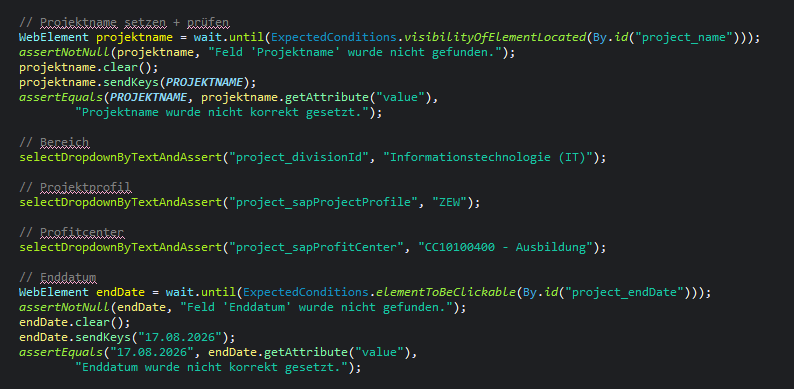
\includegraphics[width=1\textwidth]{assets/img/SeleniumCodeVs.png}
    \caption{Ausführung der Projektanlage mittels Selenium}
    \label{fig:selenium_projektanlage}
\end{figure}

Wie im Quellcode erkennbar, wird für jedes relevante Element in Selenium zunächst ein explizites Warten (Wait) definiert. Beim Feld \texttt{project\_name} wird auf die Sichtbarkeit gewartet, beim Feld \texttt{project\_endDate} auf die Klickbarkeit. Erst danach können die Felder geleert und mit den Testdaten befüllt werden. Dies macht den Code zwar robust gegenüber dynamischen Ladezeiten, erhöht jedoch die Zeilenanzahl und verleiht dem Test einen stark technischen Charakter.

% PLATZHALTER: Screenshot Cypress
\begin{figure}[H]
    \centering
    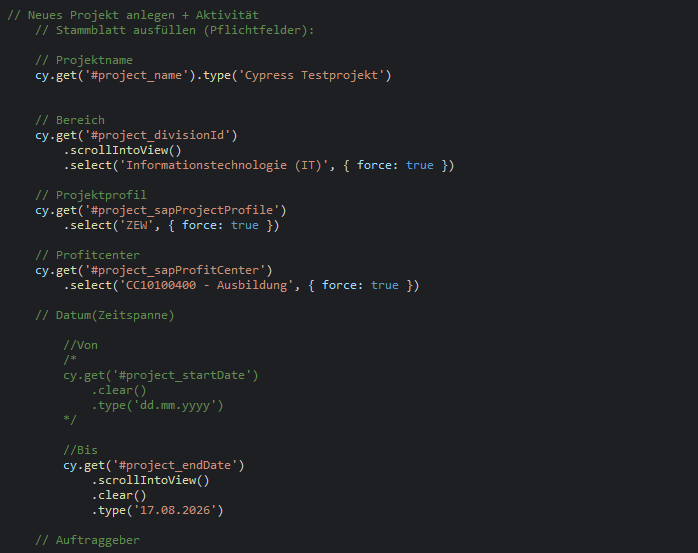
\includegraphics[width=1\textwidth]{assets/img/CypressCodeVs.png}
    \caption{Ausführung der Projektanlage im Cypress Test Runner}
    \label{fig:cypress_projektanlage}
\end{figure}

Cypress nutzt im Gegensatz dazu, wie in Quellcode \ref{lst:cypress_form} dargestellt, die Anweisung \texttt{cy.get()} zur Auswahl des Elements. Notwendige Wartebedingungen sind in den Cypress-Standardbefehlen bereits implizit integriert, sodass die Aktionen direkt verkettet (Chaining) werden können. Für das Datumsfeld wird zusätzlich \texttt{scrollIntoView()} verwendet, um sicherzustellen, dass sich das Element im sichtbaren Viewport befindet. 

Aus dieser Gegenüberstellung lassen sich folgende Bewertungsaspekte für die Nutzwertanalyse ableiten:
\begin{enumerate}
    \item \textbf{Synchronisation:} Selenium erfordert bei dynamischen Oberflächen die manuelle Definition expliziter Waits. Cypress kapselt diese Wartebedingungen in seinen Standardbefehlen.
    \item \textbf{Codeumfang:} Selenium benötigt mehr Programmzeilen, da Wartebedingungen und Elementvariablen separiert werden. Cypress erreicht durch das Chaining eine kompaktere Darstellung.
    \item \textbf{Lesbarkeit:} Der Selenium-Code ist stark technisch strukturiert. Die Cypress-Syntax liest sich hingegen eher wie eine direkte funktionale Beschreibung der Anwenderaktion.
    \item \textbf{Wartbarkeit:} Während Cypress einfache UI-Abläufe nativ kompakt hält, erfordert Selenium bei wachsendem Testumfang zwingend den Einsatz von Hilfsmethoden oder Architekturmustern (wie dem Page Object Model), um die Wartbarkeit sicherzustellen.
\end{enumerate}

Zusammenfassend zeigt der Vergleich, dass Selenium eine sehr feingranulare Steuerung der Synchronisation ermöglicht, was jedoch den Code-Overhead erhöht. Cypress bietet insbesondere bei formularbasierten Interaktionen eine lesbarere und kompaktere Syntax, was die Einarbeitung und Pflege der Tests erleichtert.
\section{Ergebnisse und Nutzwertberechnung}
\label{sec:ergebnisse}

\subsection{Präsentation der quantitativen Messdaten}
\label{subsec:messdaten}
% Gegenüberstellung der Scores (1-10) für alle Unterkriterien

\subsection{Mathematische Auswertung (Nutzwertmatrix)}
\label{subsec:nutzwertmatrix}
% Einbindung der LaTeX-Tabelle mit gewichteten Nutzwerten

\subsection{Analyse und Diskussion der Ergebnisse}
\label{subsec:diskussion}
% Interpretation: Warum Cypress trotz Setup-Hürden gewinnt / Wo Selenium punktet
% --------------------------------------------------
% 6. Fazit und Ausblick
% --------------------------------------------------

\section{Fazit und Ausblick}
\label{ch:fazit}

\subsection{Beantwortung der Forschungsfrage und Handlungsempfehlung}
\label{sec:beantwortung_forschungsfrage}

Ziel dieser Fallstudie war es zu evaluieren, welches End-to-End-Test-Framework -- Selenium oder Cypress -- sich besser für die Automatisierung regressionskritischer Testszenarien im Umfeld der JUMO GmbH \& Co. KG eignet. Die durchgeführte Nutzwertanalyse liefert hierauf eine differenzierte Antwort.

Aus rein technischer und entwicklungsorientierter Perspektive erweist sich \textbf{Cypress} als das überlegene Tool. Es punktet durch eine intuitive Syntax, exzellente Debugging-Möglichkeiten und eine signifikant höhere Stabilität bei dynamischen Webanwendungen. Die integrierten Retry-Mechanismen reduzieren die Fehleranfälligkeit bei Ladezeiten drastisch. 

Dennoch führt diese Überlegenheit nicht zu einer uneingeschränkten Empfehlung. Die infrastrukturellen Voraussetzungen der JUMO GmbH \& Co. KG basieren stark auf einem Java-Ökosystem, während Cypress eine Node.js-Umgebung erfordert. Die in der Evaluierung aufgetretenen Konflikte mit den strengen Proxy- und Sicherheitsrichtlinien des Unternehmens bremsen den Automatisierungsgewinn derzeit aus.

\textbf{Selenium} hingegen ist durch seine Java-Kompatibilität direkt und ohne administrativen Zusatzaufwand in die bestehende Infrastruktur integrierbar. Es erfordert zwar einen höheren Programmieraufwand zur Sicherstellung der Teststabilität, stellt aber unter den aktuellen Rahmenbedingungen die pragmatischere Lösung dar.

Die \textbf{Handlungsempfehlung} für das Unternehmen lautet daher: Kurzfristig sollte Selenium für die Automatisierung der regressionskritischen Tests der Puma-Anwendung genutzt werden, da die Integration in das bestehende Java-/Maven-Umfeld sofort möglich ist. Mittelfristig sollte jedoch geprüft werden, ob die IT-Infrastruktur so angepasst werden kann (z.\,B. durch Freigaben im Proxy und die Bereitstellung von Node.js in der CI/CD-Pipeline), dass ein Wechsel auf Cypress möglich wird, um von dessen überlegener Teststabilität und Entwicklerfreundlichkeit zu profitieren.

\subsection{Kritische Reflexion und Methodengrenzen}
\label{sec:reflexion}

Die in dieser Fallstudie angewandte Methodik und die daraus abgeleiteten Ergebnisse unterliegen gewissen Einschränkungen, die bei der abschließenden Bewertung zu berücksichtigen sind. 

Zunächst basiert die Bewertung der CI- und Reporting-Integration für beide Tools teilweise auf theoretischen Annahmen. Im Rahmen des zeitlich begrenzten Praxisprojekts lag der Fokus auf der prototypischen Erstellung lokaler Tests; eine vollständige Integration in eine automatisierte Build-Pipeline wurde nicht abschließend praktisch umgesetzt. Des Weiteren ist zu beachten, dass qualitative Bewertungskriterien wie \textit{Lesbarkeit der Syntax} und \textit{Usability des Test Runners} zwangsläufig einer subjektiven Wahrnehmung des Evaluierenden unterliegen, auch wenn sie durch konkrete Implementierungserfahrungen untermauert wurden.

Abschließend ist eine klare fachliche Differenzierung bezüglich der identifizierten Schwächen von Cypress notwendig: Die gravierendsten Punktabzüge, welche bei der Projekterstellung und Installation auftraten, stellen keine originären Schwächen des Tools dar. Sie resultieren vielmehr maßgeblich aus den rigiden Sicherheits- und Proxy-Richtlinien der Unternehmensinfrastruktur. Würde das Unternehmen standardmäßig Node.js-Umgebungen und entsprechende Paket-Freigaben unterstützen, fiele die Nutzwertanalyse noch deutlicher zugunsten von Cypress aus.

\subsection{Ausblick}
\label{sec:ausblick}

Zukünftige Arbeiten könnten die in dieser Fallstudie identifizierten Einschränkungen aufgreifen. Eine logische Fortführung wäre die praktische Implementierung beider Frameworks in einer vollständigen CI/CD-Pipeline (z.\,B. Jenkins oder GitLab CI), um die theoretischen Annahmen zur Reporting- und Ausführungsfähigkeit im automatisierten Build-Prozess empirisch zu belegen. 

Darüber hinaus sollte das Unternehmen die strategische Entscheidung treffen, inwiefern moderne JavaScript-/TypeScript-basierte Testing-Tools zukünftig gefördert werden sollen, um langfristig die Effizienz in der Qualitätssicherung von Webanwendungen zu steigern.

% Literatur
\newpage
\setstretch{1} % andere Zeilenhöhe
\normalsize
\printbibliography[title={Literaturverzeichnis}]
\addcontentsline{toc}{section}{Literaturverzeichnis} 
\markboth{Literaturverzeichnis}{Literaturverzeichnis}

% Glossar und Abkürzungsverzeichn
\printnoidxglossary[title=Glossar, toctitle=Glossar]

\printnoidxglossary[type=\acronymtype, title=Abkürzungsverzeichnis, toctitle=Abkürzungsverzeichnis]




\section*{Eigenständigkeitserklärung}
\addcontentsline{toc}{section}{Eigenständigkeitserklärung}
Hiermit erkläre ich, dass ich die vorliegende Arbeit selbstständig verfasst und keine anderen als die angegebenen Quellen und Hilfsmittel benutzt habe. 

Alle sinngemäß und wörtlich übernommenen Textstellen aus fremden Quellen wurden kenntlich gemacht.\\[2cm]
Fulda, den 17.08.2026 \\[1.5cm]
\rule{6cm}{0.4pt}\\
Marcel Licht
\clearpage


%%%%%%%%%%%%%%%%%%%%%%
%%%%% ~~~~~ Anhang
%%%%%%%%%%%%%%%%%%%%%%
% Anhangeinstellungen
\renewcommand{\appendixtocname}{Anhänge}
\renewcommand{\appendixpagename}{Anhang}
\appendix
\addappheadtotoc


\section{Erklärung zur Nutzung von KI-Werkzeugen}
%\addcontentsline{toc}{section}{Erklärung zur Nutzung von KI-Werkzeugen}

Bei der Erstellung dieses Exposés wurden KI-Werkzeuge unterstützend genutzt:

Verwendete Tools: Google Gemini 3.1 Pro

\begin{itemize}
    \item Hilfe bei der sprachlichen Überarbeitung und Verbesserung eigener Texte (Formulierungshilfe, Grammatik, und Rechtschreibprüfung)
    \item Hilfe bei LaTeX Befehlen und Formatierungen (z.B. Quellen in der references.bib oder Tabelle)
    \item Überprüfung auf Vollständigkeit der Anforderungen
    \item Unterstützung bei der Literaturrecherche
\end{itemize}

\section{Bewertungsmatrix (Excel)}
\label{sec:anhang_bewertungsmatrix}

In diesem Abschnitt ist die vollständige Bewertungsmatrix der Nutzwertanalyse abgebildet, die als Grundlage für die finale Auswertung diente. Aufgrund des Umfangs der Kriterien und Begründungen wurde die Darstellung der Excel-Datei in zwei Abbildungen aufgeteilt.

\begin{figure}[htbp]
    \centering
    % Passe den Dateinamen an deine Screenshots an
    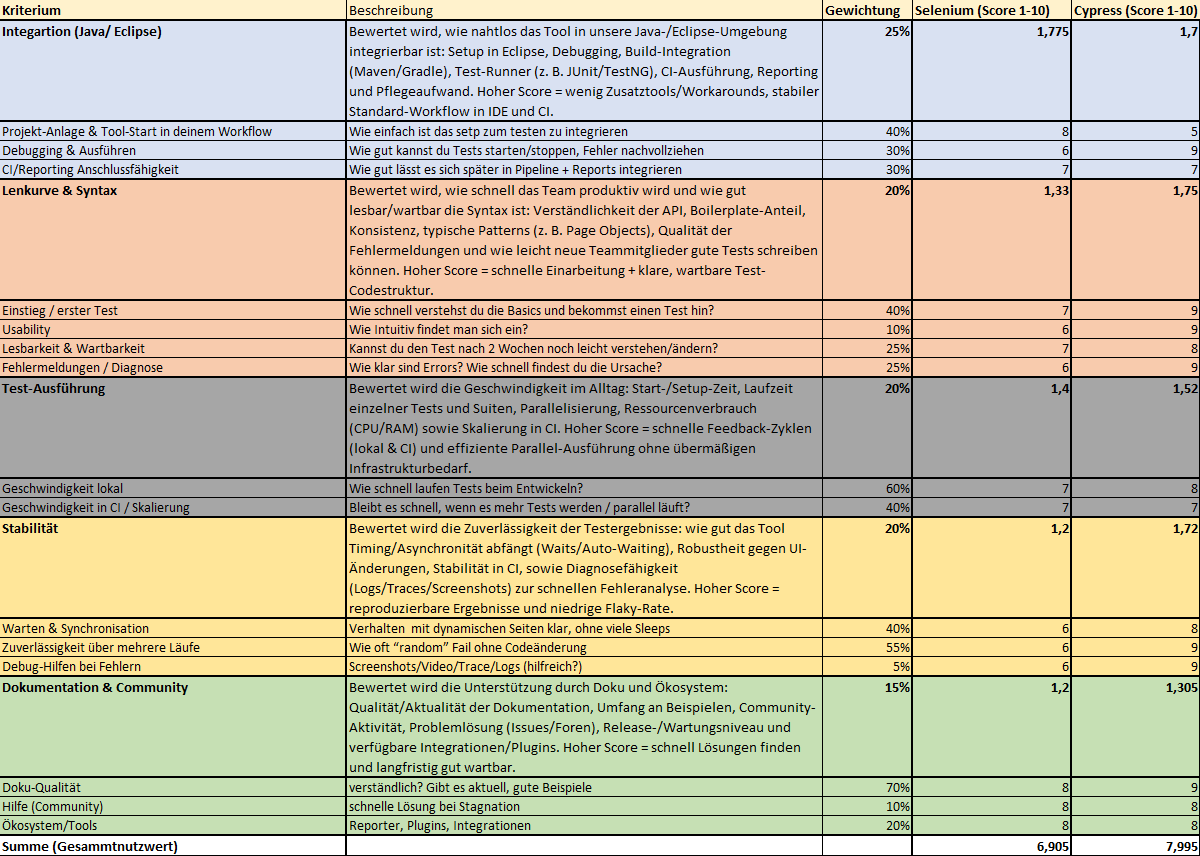
\includegraphics[width=\textwidth]{assets/img/BewertungsmatrixAusgefüllt.png}
    \caption{Bewertungsmatrix der Nutzwertanalyse (Selenium vs. Cypress) -- Teil 1}
    \label{fig:bewertungsmatrix_1}
\end{figure}

\begin{figure}[htbp]
    \centering
    % Passe den Dateinamen an deine Screenshots an
    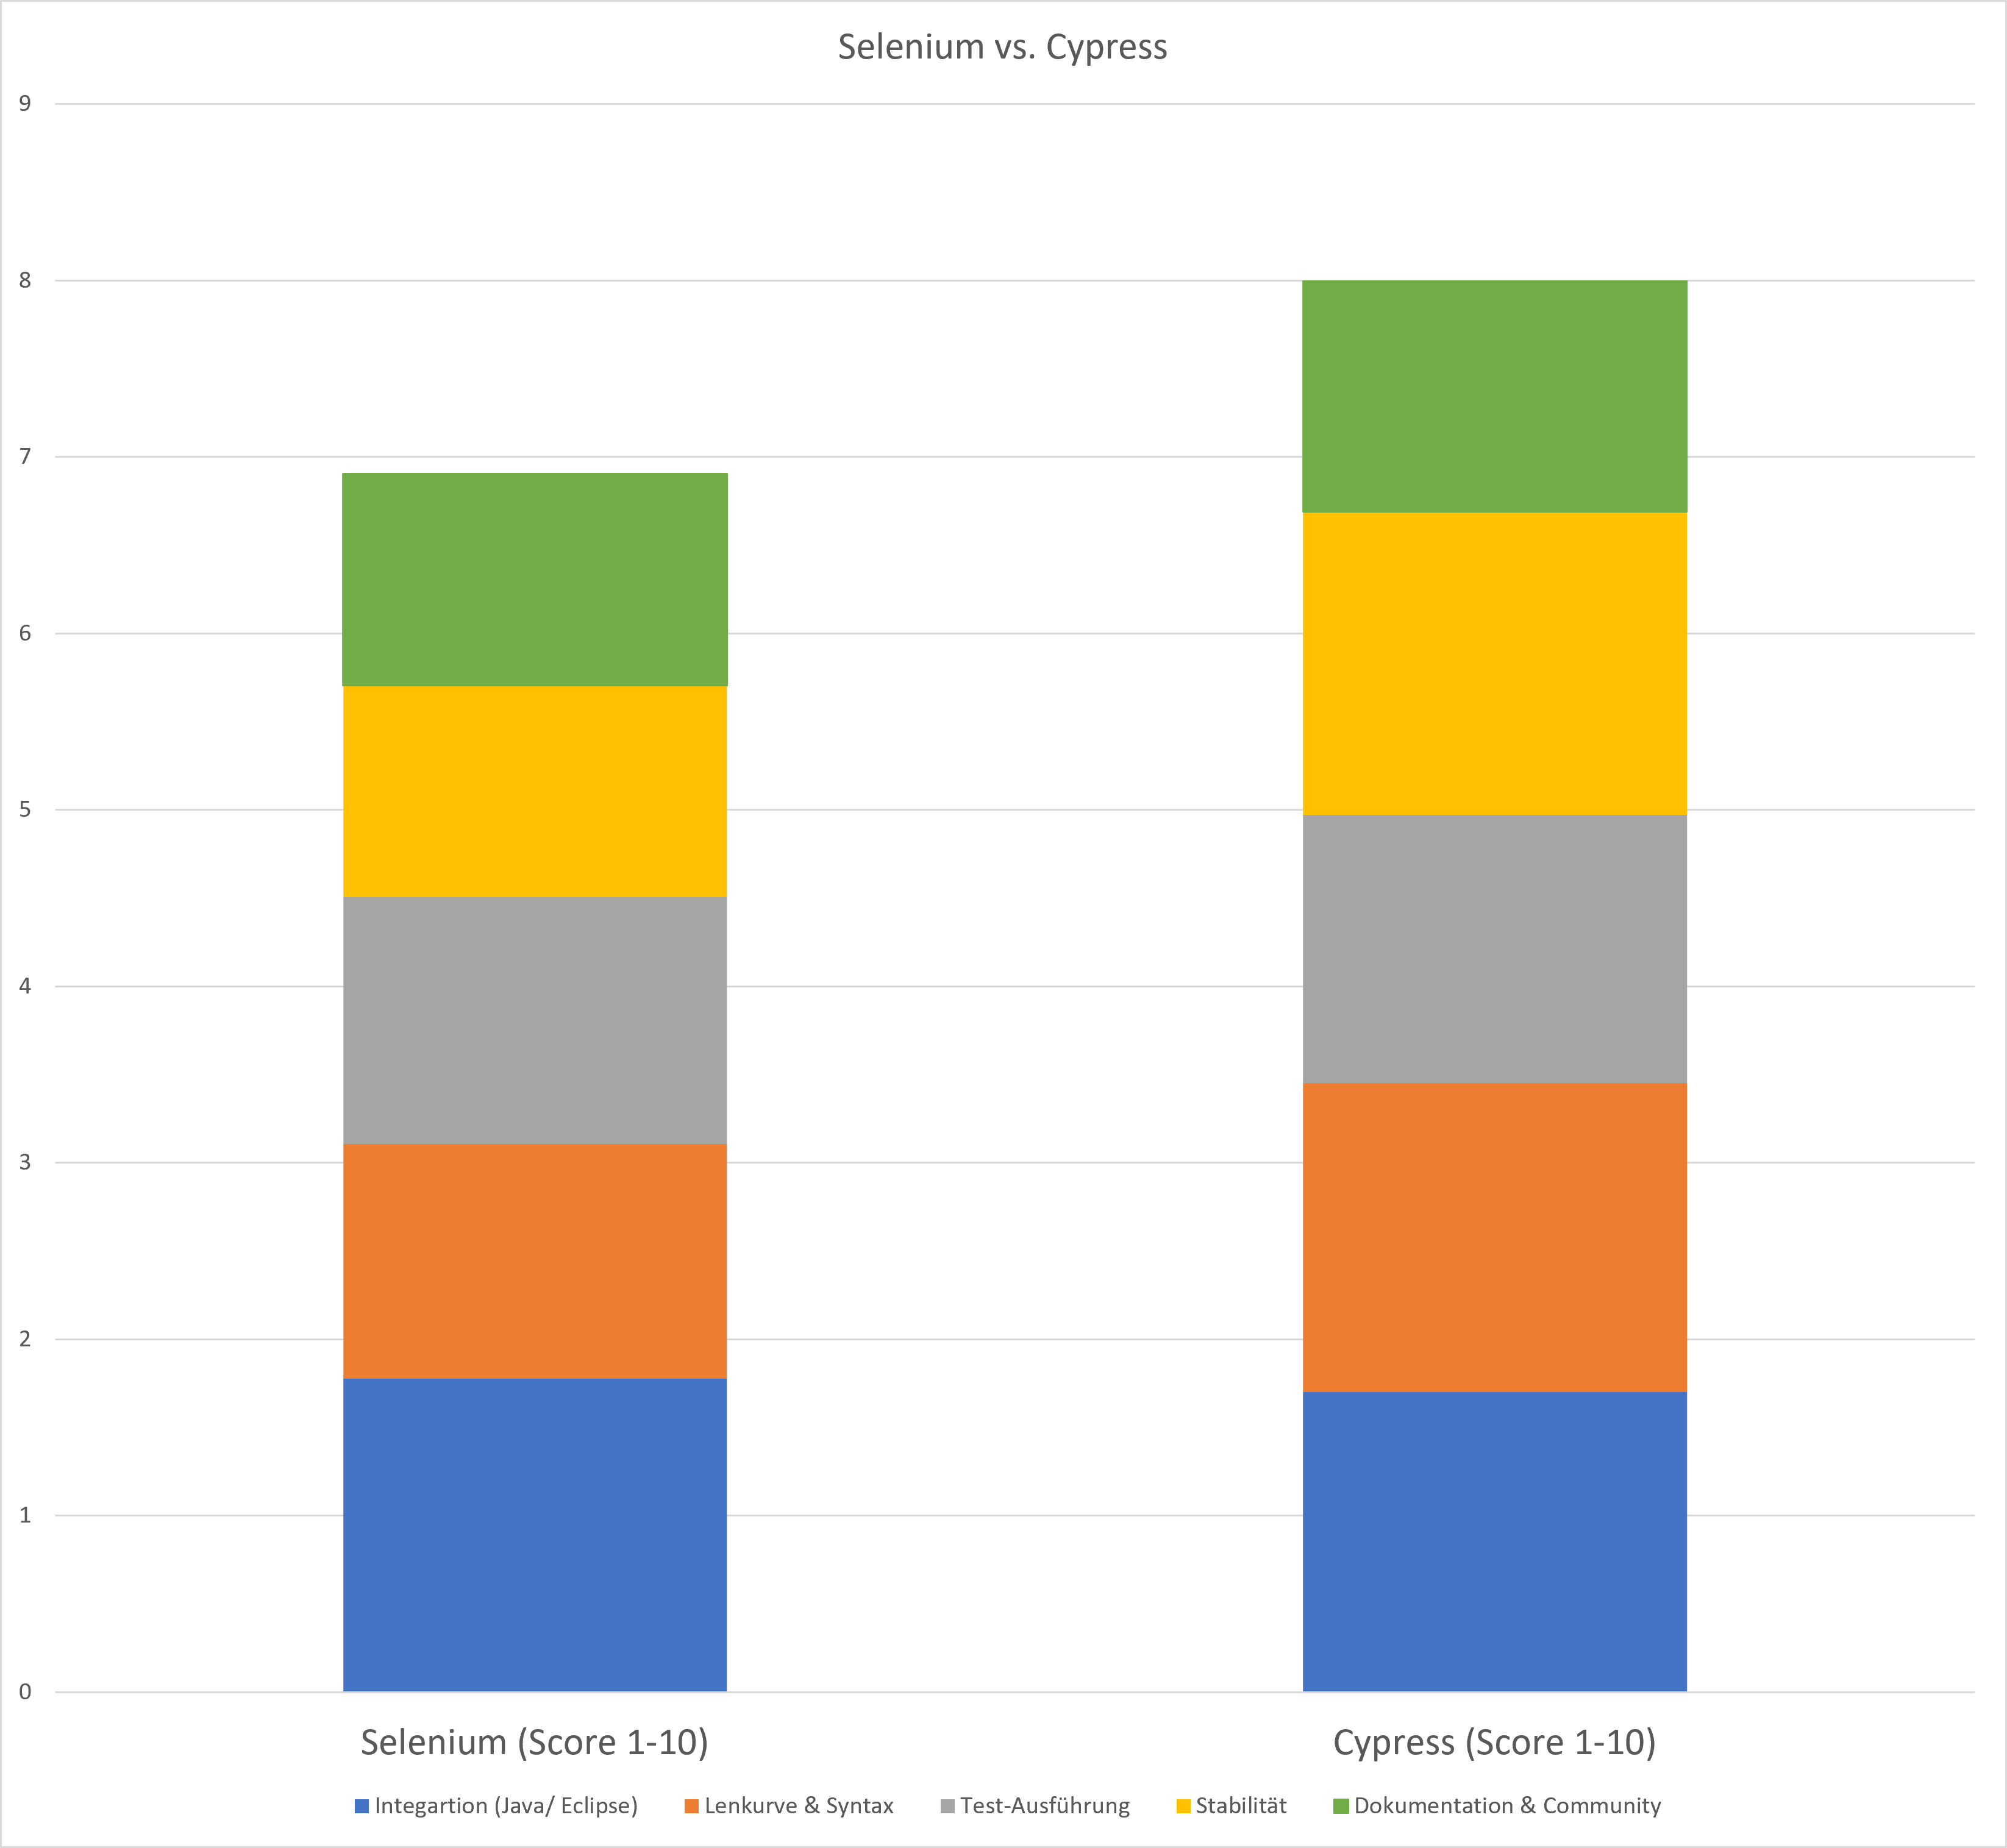
\includegraphics[width=\textwidth]{assets/img/DiagrammSelVsCy.png}
    \caption{Bewertungsmatrix der Nutzwertanalyse (Selenium vs. Cypress) -- Teil 2}
    \label{fig:bewertungsmatrix_2}
\end{figure}

\section{TestLog}


% Ende Dokument
\end{document}
